% Row-normalised confusion matrix of the INT8 thread classifier on the 10,563 synthetic test threads
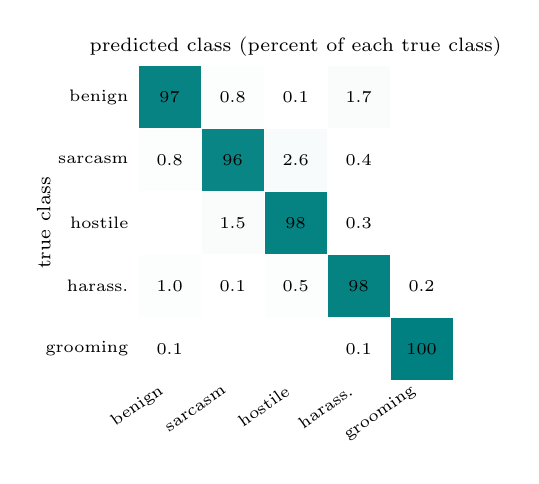
\begin{tikzpicture}[x=0.8cm,y=0.8cm]
  \foreach \i/\j/\c/\lab in {0/0/97/{97},0/1/1/{0.8},0/2/0/{0.1},0/3/2/{1.7},0/4/0/{},1/0/1/{0.8},1/1/96/{96},1/2/3/{2.6},1/3/0/{0.4},1/4/0/{},2/0/0/{},2/1/2/{1.5},2/2/98/{98},2/3/0/{0.3},2/4/0/{},3/0/1/{1.0},3/1/0/{0.1},3/2/1/{0.5},3/3/98/{98},3/4/0/{0.2},4/0/0/{0.1},4/1/0/{},4/2/0/{},4/3/0/{0.1},4/4/100/{100}}{
    \pgfmathsetmacro{\yy}{-\i}
    \node[draw=white, fill=teal!\c!white, minimum width=0.8cm, minimum height=0.8cm, inner sep=0pt,
          font=\fontsize{6.5}{7}\selectfont, text=black] at (\j,\yy) {\lab};
  }
  \foreach \k/\n in {0/benign,1/sarcasm,2/hostile,3/harass.,4/grooming}{
    \node[font=\fontsize{6.5}{7}\selectfont, anchor=east] at (-0.5,-\k) {\n};
    \node[font=\fontsize{6.5}{7}\selectfont, rotate=35, anchor=east] at (\k,-4.55) {\n};
  }
  \node[font=\fontsize{7}{8}\selectfont, rotate=90] at (-2.0,-2) {true class};
  \node[font=\fontsize{7}{8}\selectfont] at (2,0.8) {predicted class (percent of each true class)};
\end{tikzpicture}
